\documentclass[a4paper,11pt]{article}
\usepackage[a4paper,total={18cm, 24cm}]{geometry}
\usepackage[parfill]{parskip}
\usepackage[utf8]{inputenc}
\usepackage[T1]{fontenc}
\usepackage{fancyhdr}
\usepackage[ddmmyyyy]{datetime}
\usepackage{graphicx}
\usepackage{subcaption}
\usepackage{multirow}
\usepackage{hyperref}
\usepackage{amsfonts}

\pagestyle{fancy}
\fancyhf{}
\lhead{\today}
\chead{Deep Learning - Gaussian Variational Autoencoder}
\rhead{Jakub Rada}

\begin{document}
In this assignment we focus on Gaussian Variational Autoencoders.
We want to train them on the MNIST dataset and try if they can generate new reasonable images.
We will try a \textit{vanilla} versions, where the encoder and decoder are a single layer and also deeper variants with more layers.
These different models will be compared by various means.

\section*{Implementation and training (assignments 1 and 2)}
First, we implemented the VAE model as hinted on the website.
All the code for models and training is in \texttt{models.py}.
The VAE is implemented that it takes an optional list of hidden layer sizes for both the encoder and decoder, which is by default empty.

In the end, we trained multiple models with different depth and hidden layer sizes for both encoder and decoder.
However, we always made the encoder and decoder symmetric, i.e. the encoder and decoder have the same hidden layer sizes just in a reverse order.
The parameters shared all the models and the training are shown in table \ref{tab:training_params}.

\begin{table}[ht]
    \centering
    \begin{tabular}{| l | c |}
        \hline
        \textbf{parameter}     & \textbf{value} \\
        \hline
        \hline
        latent space dimension & 64             \\
        \hline
        learning rate          & $3e^{-4}$      \\
        \hline
        epochs                 & 100            \\
        \hline
        batch size             & 16             \\
        \hline
        validation split       & 0.2            \\
        \hline
    \end{tabular}
    \caption{Training parameters for all models}
    \label{tab:training_params}
\end{table}

After training the models, we display the learning curve in figure \ref{fig:learning_curve} for all models and summarize parameter sizes and other statistics in table \ref{tab:parameters}.

\begin{figure}[ht]
    \centering
    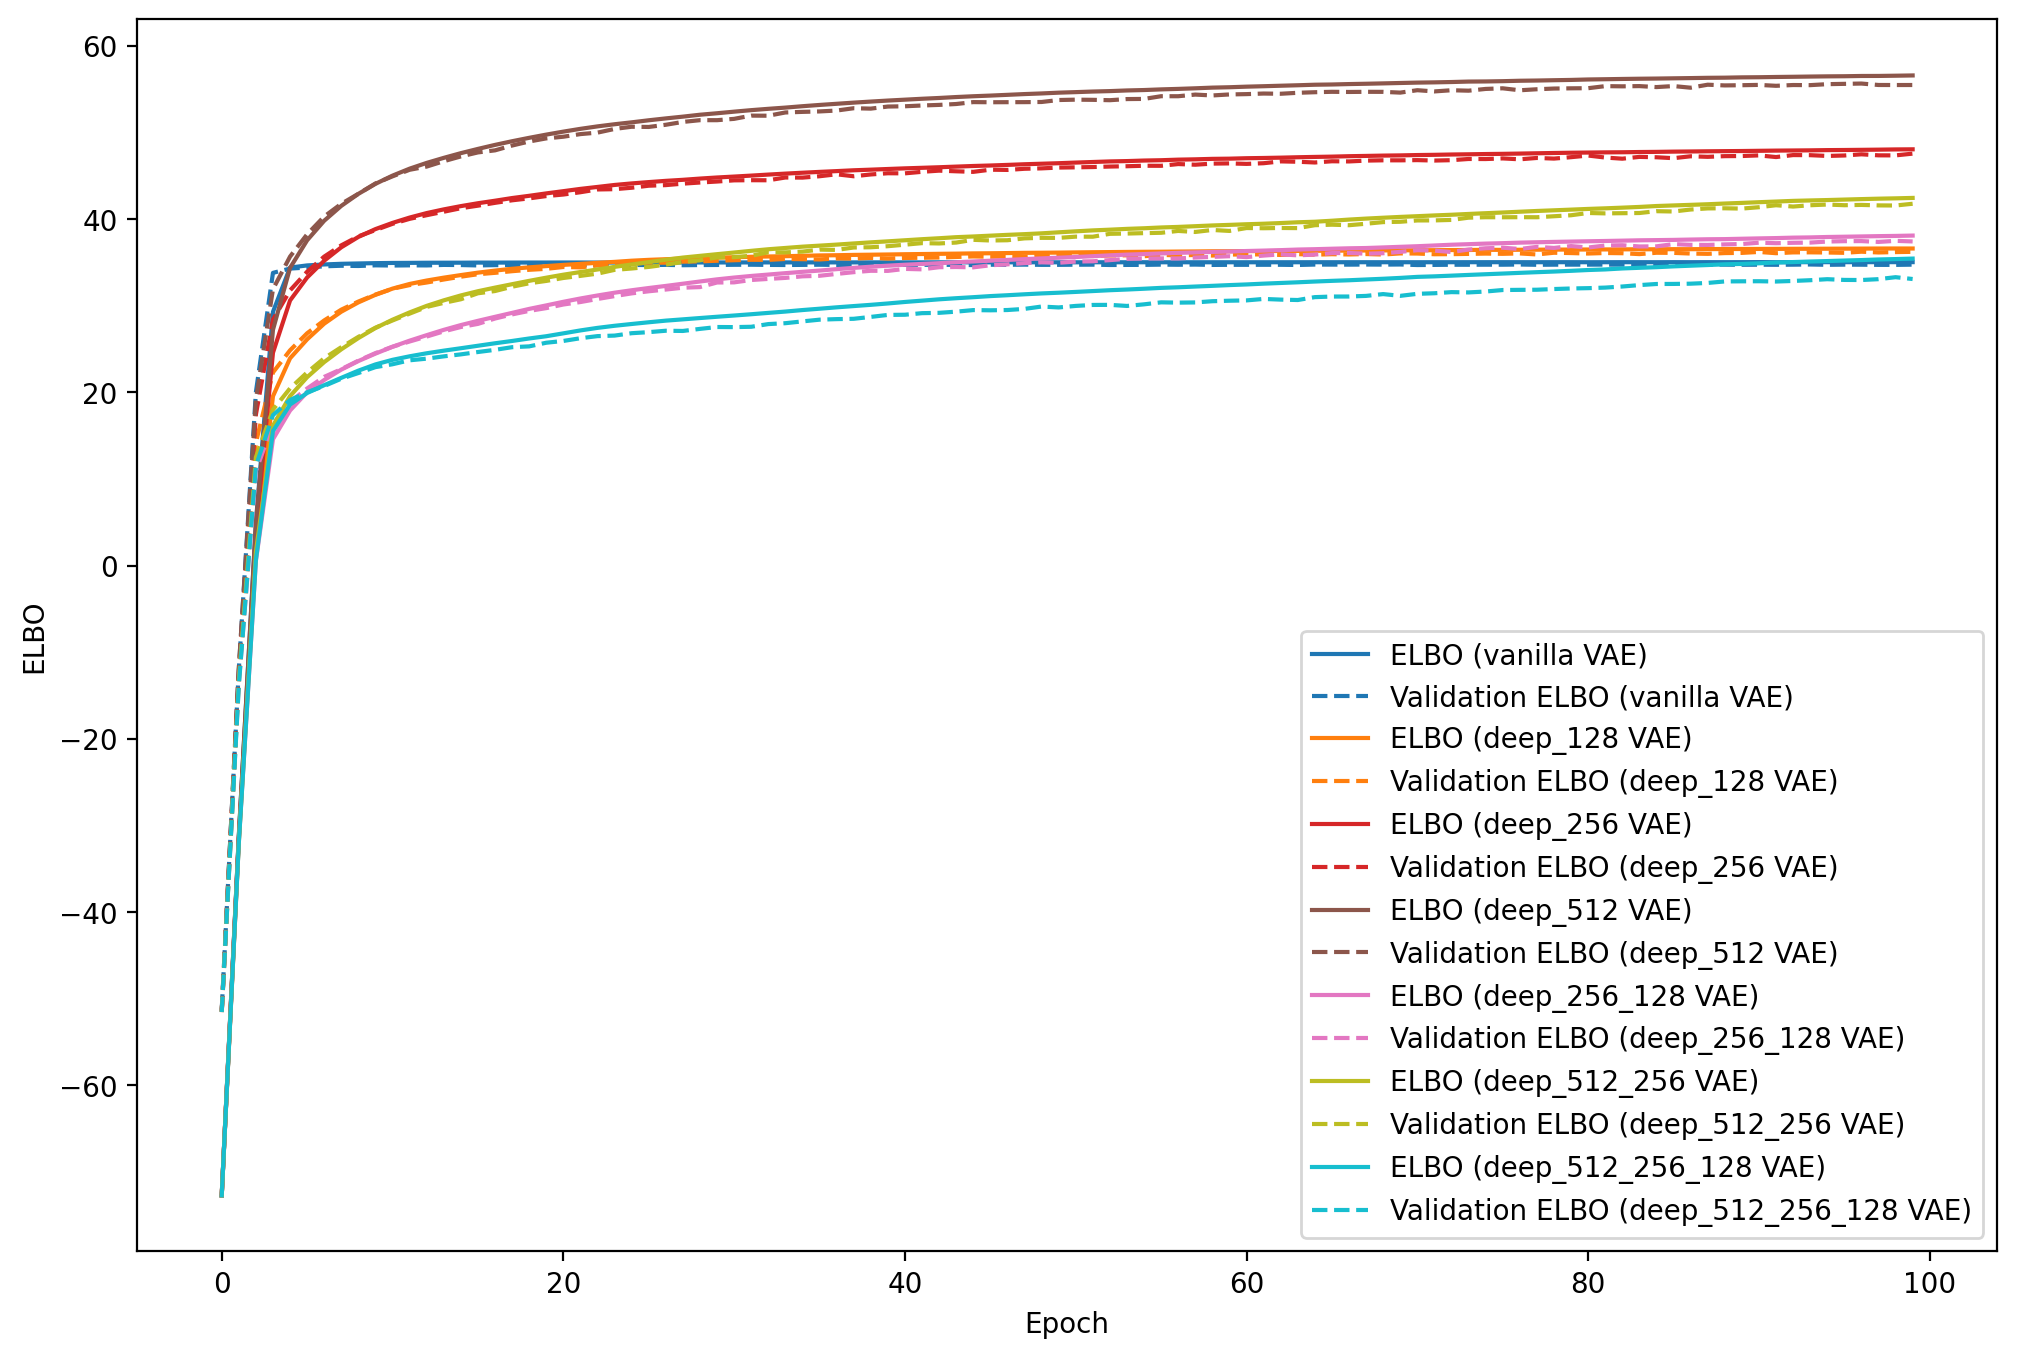
\includegraphics[width=0.8\textwidth]{../images/learning_curve.png}
    \caption{Learning curve for both training and validation sets }
    \label{fig:learning_curve}
\end{figure}

From the curves, we can observe some interesting things.
First, the learning curves of all deep models have almost exactly the same shape, they differ only in the speed of learning in the first few iterations, then they seem to follow similar trends.
In the contrary, the vanilla model with only a single linear layer learns really fast to a value of ELBO around $35$ and then it basically stops learning.

Another interesting observation is that the validation loss follows exactly the training loss for all models, which is different from what we usually see in classification tasks.
Also, all the deeper models look like they could learn further, especially the models with more layers.

The model with a single hidden layer but most hidden units reached the highest value of ELBO compared to the other models with a single hidden layer but fewer units.

\begin{table}
    \centering
    \begin{tabular}{| l | c | c || c |}
        \hline
        \textbf{type} & \textbf{encoder}                                                     & \textbf{decoder}                                                     & \textbf{number of parameters} \\
        \hline
        \hline
        vanilla       & $784 \rightarrow 64$                                                 & $64 \rightarrow 784$                                                 & $151441$                      \\
        \hline
        deep          & $784 \rightarrow 128 \rightarrow 64$                                 & $64 \rightarrow 128 \rightarrow 784$                                 & $226449$                      \\
        \hline
        deep          & $784 \rightarrow 256 \rightarrow 64$                                 & $64 \rightarrow 256 \rightarrow 784$                                 & $451985$                      \\
        \hline
        deep          & $784 \rightarrow 512 \rightarrow 64$                                 & $64 \rightarrow 512 \rightarrow 784$                                 & $903057$                      \\
        \hline
        deep          & $784 \rightarrow 256 \rightarrow 128 \rightarrow 64$                 & $64 \rightarrow 128 \rightarrow 256 \rightarrow 784$                 & $493201$                      \\
        \hline
        deep          & $784 \rightarrow 512 \rightarrow 256 \rightarrow 64$                 & $64 \rightarrow 256 \rightarrow 512 \rightarrow 784$                 & $1116561$                     \\
        \hline
        deep          & $784 \rightarrow 512 \rightarrow 256 \rightarrow 128 \rightarrow 64$ & $64 \rightarrow 128 \rightarrow 256 \rightarrow 512 \rightarrow 784$ & $1157777$                     \\
        \hline
    \end{tabular}
    \caption{Model parameters}
    \label{tab:parameters}
\end{table}

The final task in this part is displaying a tableau of $16$ images and their reconstructions by the different VAEs.
We have compiled them into a grid in Figure \ref{fig:reconstructions}, where each row represents a single image and every column represents a different model.
It is quite large but hopefully it is still readable.

From the tableau we can see that all the models reconstruct the images well, some models produce more blurry images than others.
Even the vanilla model can reconstruct the images but the blur is quite hight.
On the other hand, the model with one layer with $512$ units seems to produce the sharpest images, maybe together with the model with three layers (last column).

\begin{figure}[ht]
    \centering
    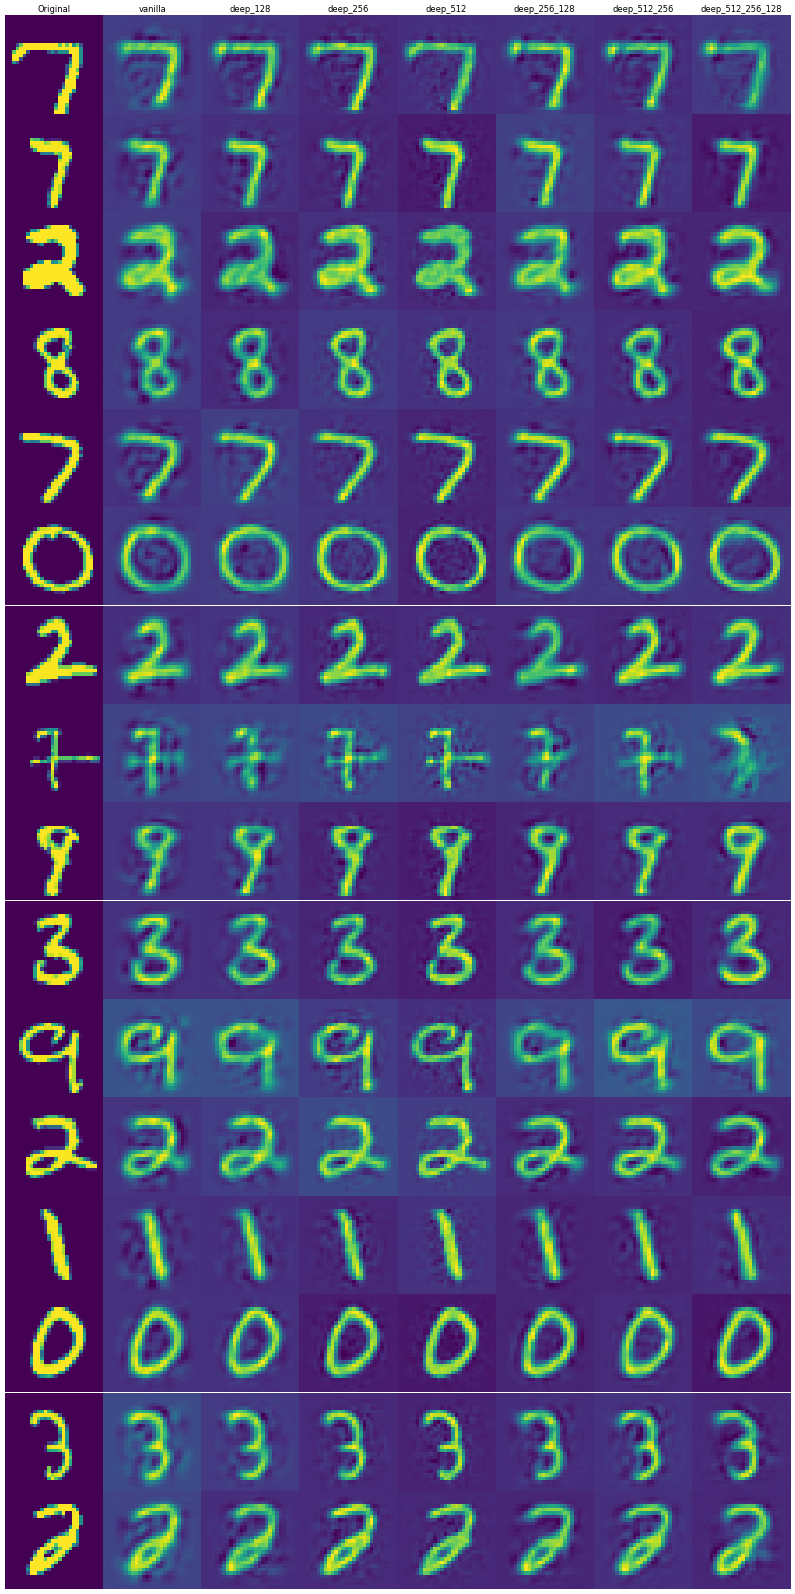
\includegraphics[width=0.6\textwidth]{../images/reconstructions.png}
    \caption{Reconstructed images from the test set by different models. From left to right: original images, vanilla model, deep 128, deep 256, deep 512, deep 256-128, deep 512-256, deep 512-256-128.}
    \label{fig:reconstructions}
\end{figure}

\clearpage

\section*{Model comparison (assignment 3)}
After successful training and verifying that the VAE can reconstruct images from the test set, we can compare the different models by using differnt metrics and comparisons.

\paragraph{ELBO} First, we compare the values of ELBO on the test set in table \ref{tab:elbo}.

\begin{table}[ht]
    \centering
    \begin{tabular}{| l | c |}
        \hline
        \textbf{model}       & \textbf{ELBO} \\
        \hline
        \hline
        vanilla              & $35.60$       \\
        \hline
        deep ($128$)         & $37.00$       \\
        \hline
        deep ($256$)         & $48.29$       \\
        \hline
        deep ($512$)         & $56.41$       \\
        \hline
        deep ($256-128$)     & $38.20$       \\
        \hline
        deep ($512-256$)     & $42.53$       \\
        \hline
        deep ($512-256-128$) & $33.79$       \\
        \hline
    \end{tabular}
    \caption{ELBO values on the test set}
    \label{tab:elbo}
\end{table}

The highest value was achieved by the model with one layer and $512$ hidden units, which corresponds to the observation from the learning curve.
However, the direct comparison between models of different number of layers and sizes might not be accurate, in my opinion, because for example the last model with the most layers in encoder and decoder has the lowest achieved ELBO, but the images are among the sharpest produced.
In training we were optimizing a lower bound which might explain this phenomenon.

\paragraph{Posterior collapse} By averaging the KL divergence over a batch of images, we can estimate which posteriors carry information and which collapse.
For comparison I show only a couple of the above mentioned models to avoid cluttering the report with too many images, see \ref{fig:collapse}.

\begin{figure}[ht]
    \centering
    \begin{subfigure}[t]{0.3\textwidth}
        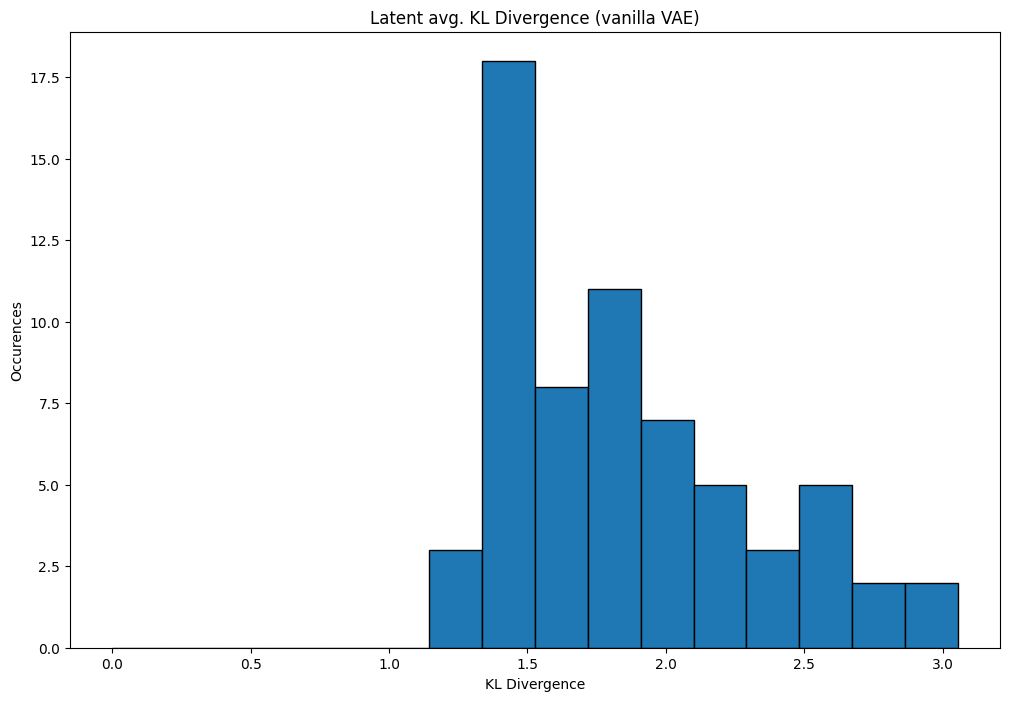
\includegraphics[width=\textwidth]{../images/collapse_vanilla.png}
        \caption{Vanilla model}
    \end{subfigure}
    \hfill
    \begin{subfigure}[t]{0.3\textwidth}
        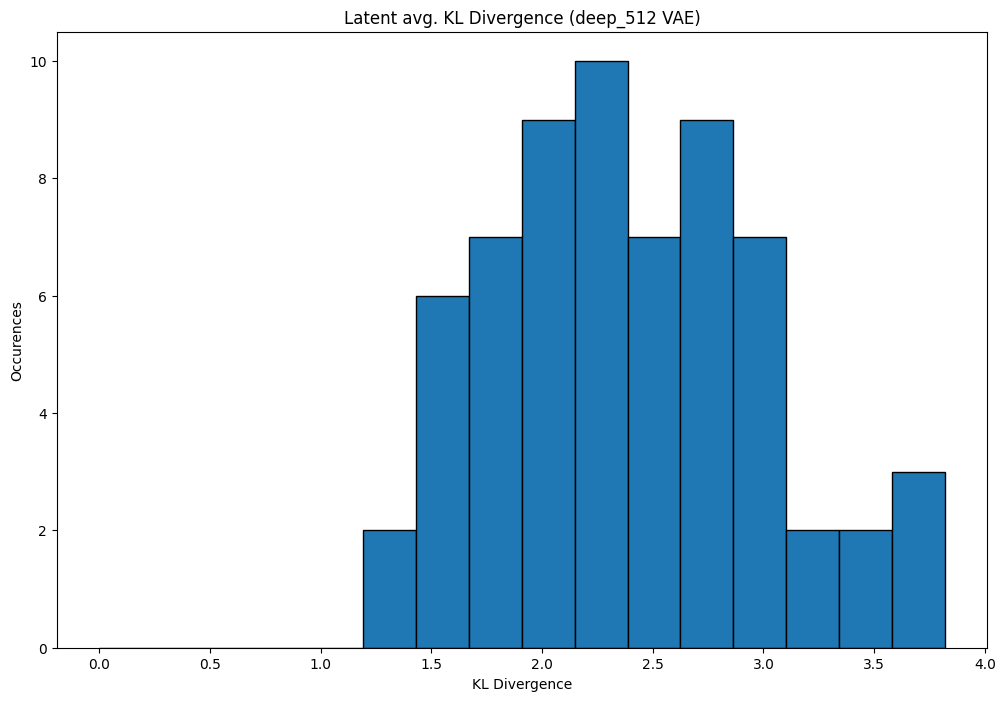
\includegraphics[width=\textwidth]{../images/collapse_512.png}
        \caption{Deep model with one layer and $512$ hidden units}
    \end{subfigure}
    \hfill
    \begin{subfigure}[t]{0.3\textwidth}
        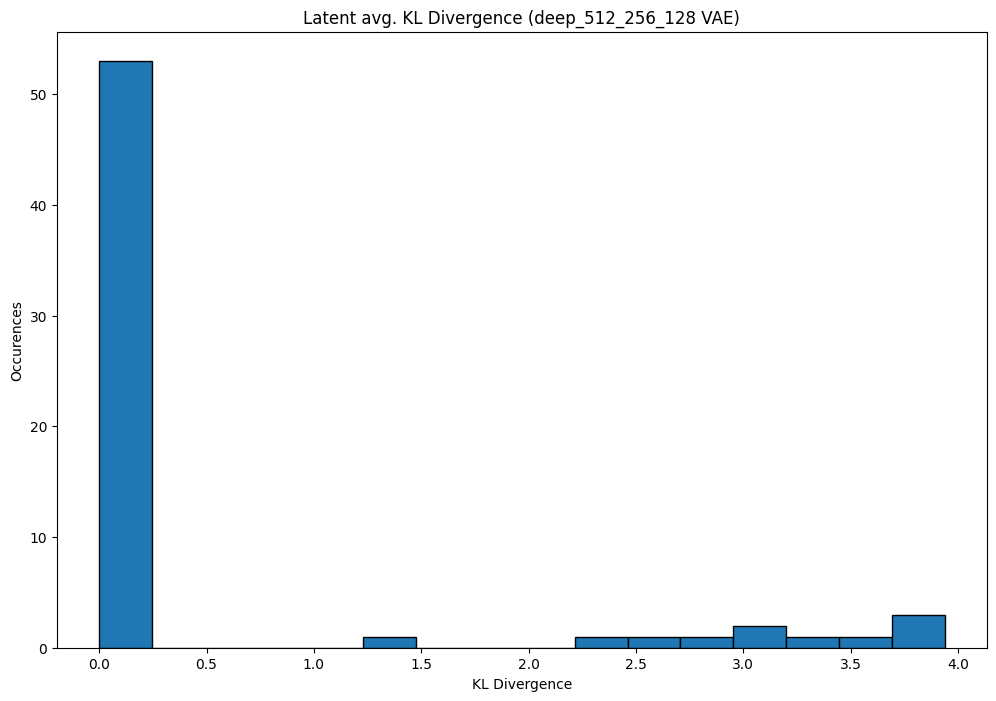
\includegraphics[width=\textwidth]{../images/collapse_512_256_128.png}
        \caption{Deepest model with three layers of $512-256-128$ hidden units}
    \end{subfigure}
    \caption{Posterior collapse in the latent dimension for some models}
    \label{fig:collapse}
\end{figure}

Interestingly, the vanilla model does not have any collapsed posteriors, similarly to the model with $512$ hidden units.
All other models I trained have some, the most collapsed posteriors are in the model with $512-256-128$ hidden units as seen in the histograms.
In the next part, we will compare the models on generating images and we will can see if this has an effect on the performance.

\paragraph{Decoder evaluation} Now we want to compare the generative ability of the decoder part of the VAE on noise sampled from $\mathcal{N}(0, 1)$.
Again, we display only some of the models to avoid too many images, see \ref{fig:generations}.

\begin{figure}[ht]
    \centering
    \begin{subfigure}[t]{0.35\textwidth}
        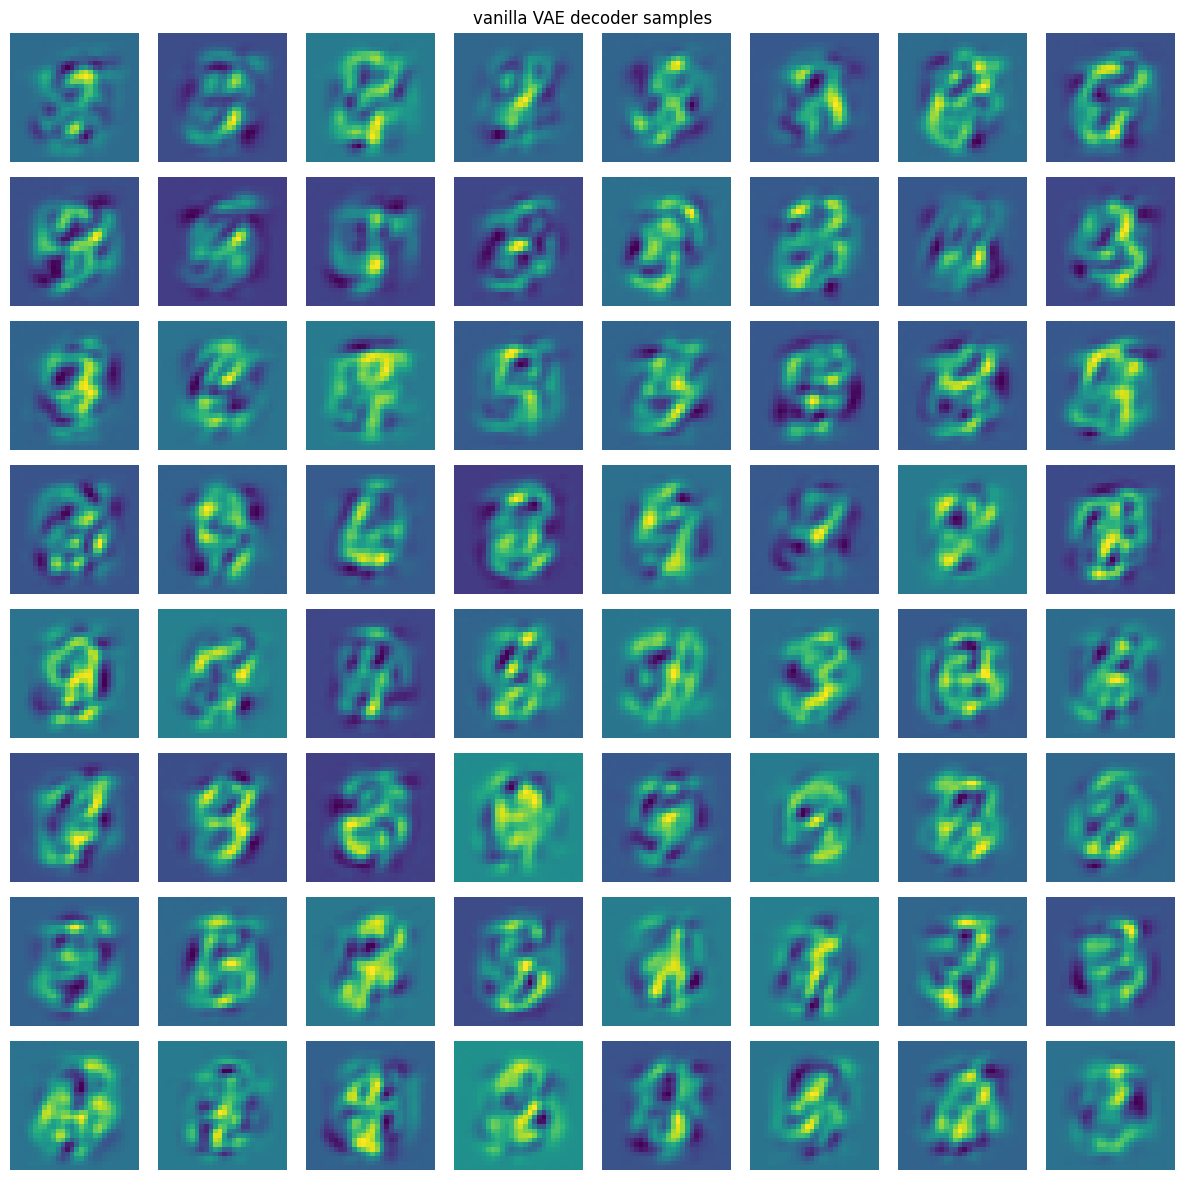
\includegraphics[width=\textwidth]{../images/decoder_vanilla.png}
        \caption{Vanilla model}
    \end{subfigure}
    \hfill
    \begin{subfigure}[t]{0.35\textwidth}
        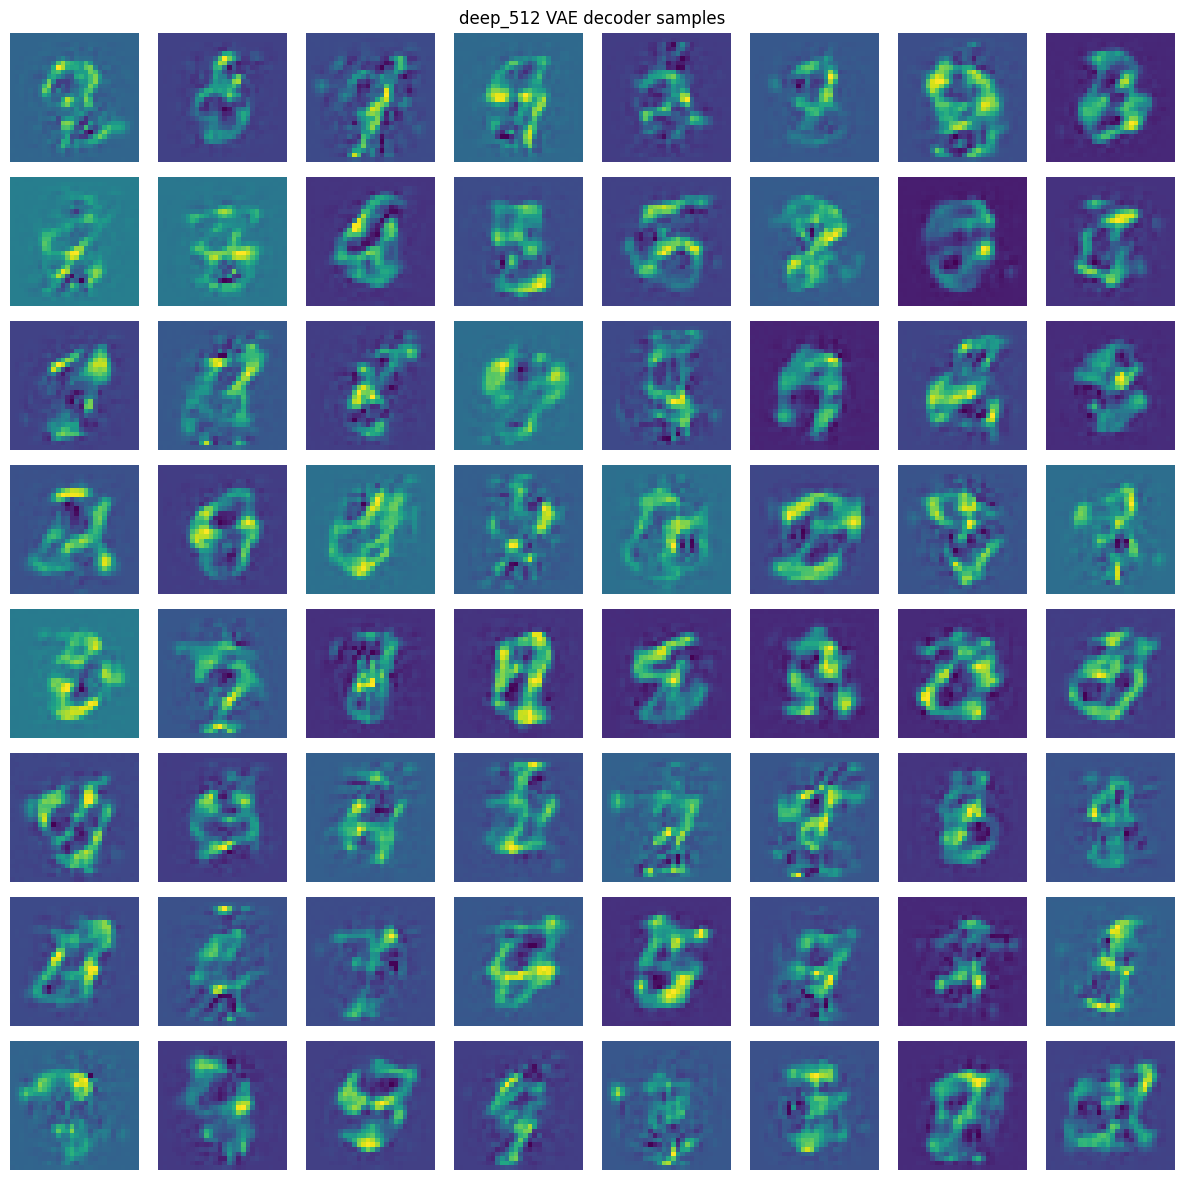
\includegraphics[width=\textwidth]{../images/decoder_512.png}
        \caption{Deep model with one layer and $512$ hidden units}
    \end{subfigure}
    \begin{subfigure}[t]{0.35\textwidth}
        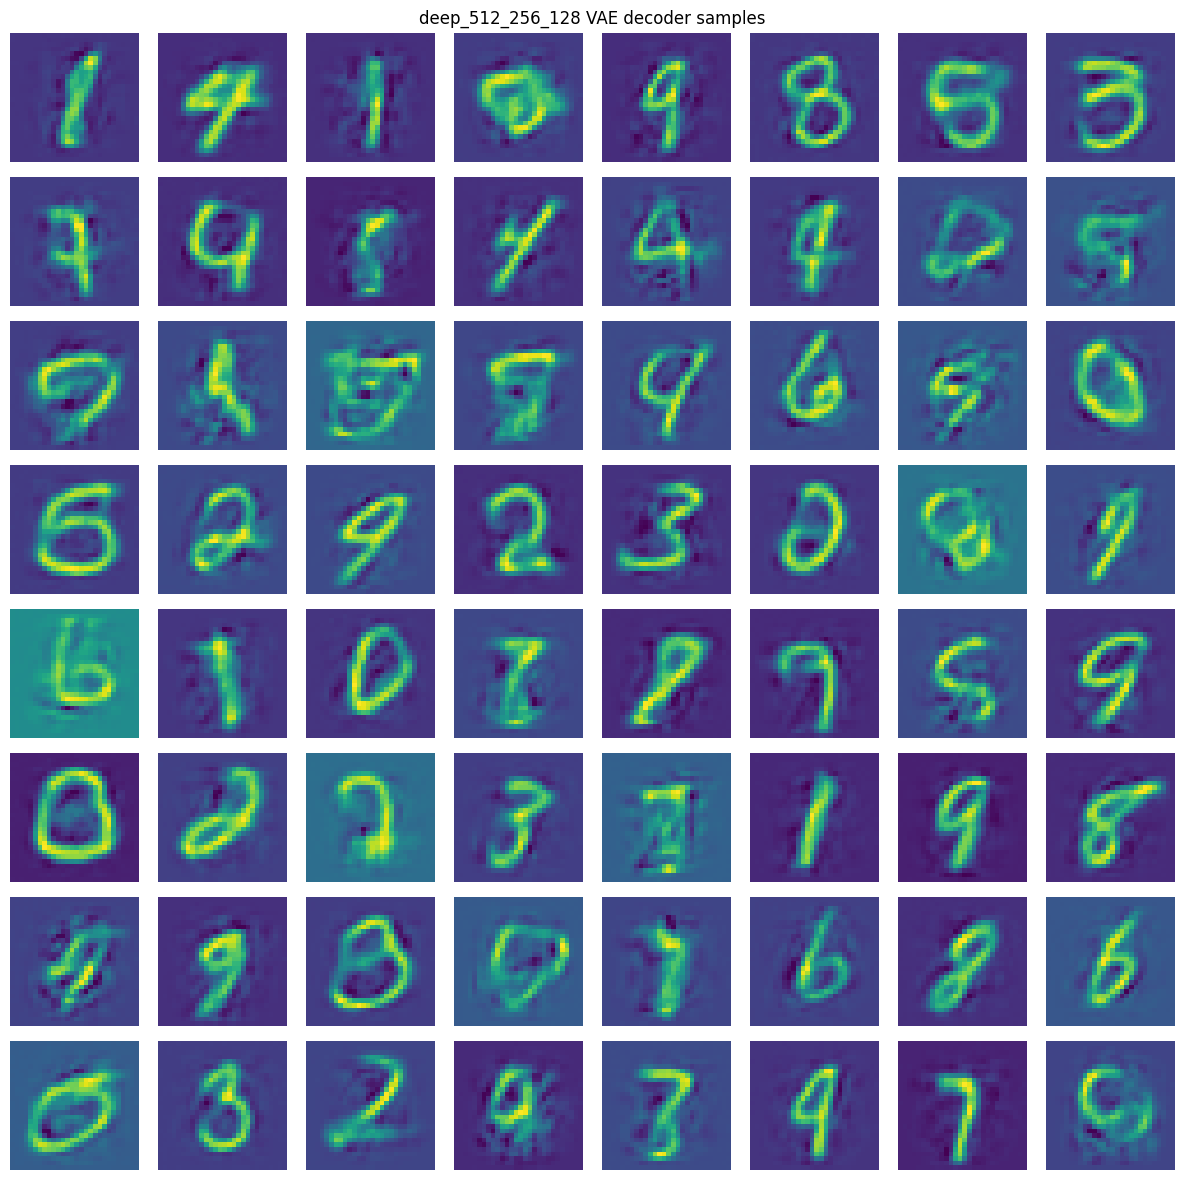
\includegraphics[width=\textwidth]{../images/decoder_512_256_128.png}
        \caption{Deepest model with three layers of $512-256-128$ hidden units}
    \end{subfigure}
    \caption{Images generated by decoders from $\mathcal{N}(0, 1)$ for some models}
    \label{fig:generations}
\end{figure}

We can observe some interesting things from the generated images.
Even though the deepest model has the lowest ELBO and the most collapsed posteriors, it generated images that are somewhat similar to the training images from MNIST.
The other models produce only some mixture of different numbers and most of the time it is impossible to say that the image is indeed a number.
So maybe just using ELBO and collapsed posteriors is not enough to evaluate the quality of a model.
Also, it might be the case that the depth of the decoder matters much for the quality of generated images.

\clearpage

\paragraph{Limiting distribution} While implementing this last step we faced some problems with the trained models.
It happened to us that the standard deviation predicted by the decoder was either so small or so big that when taken in the exponential, it collapsed to zero or infinity, which caused troubles in sampling from the normal distribution.
We tried to fix this issue by either normalizing the generated images in each step to $[0, 1]$ or by clipping the predicted standard deviation to some fixed range before applying the exponential but both these approaches led to bad results.
The result of the $100$ steps resulted in images filled with all ones or close to all ones.

We tried to tune some parameters of the learning and found out that if training the models on batches of size $64$ rather than $16$, the problem disappears.
Moreover, we added the kaiming initialization to the weights of the decoder and encoder to further regularize learning, even though the networks are not really deep.
One of these or a combination fixed the problem, so now we will showcase some results and comparisons again but for the retrained models.
Also, the limiting distribution will be shown only for the retrained models as we were not able to produce meaningful results with the originally trained models.
It is unclear to us why the batch of $16$ images is problematic, from the lectures it seemed that it serves as implicit regularization so the models should generalize better.
But maybe it is something specific to VAEs or the domain.

\section*{Retraining the models on batches of size $64$}
In the retraining, everything is the same as in the original training (Table \ref{tab:training_params}) except for the batch size which is now $64$ and the added advanced initialization.
The learning curves are shown again all together in Figure \ref{fig:64_learning_curve}.

\begin{figure}[ht]
    \centering
    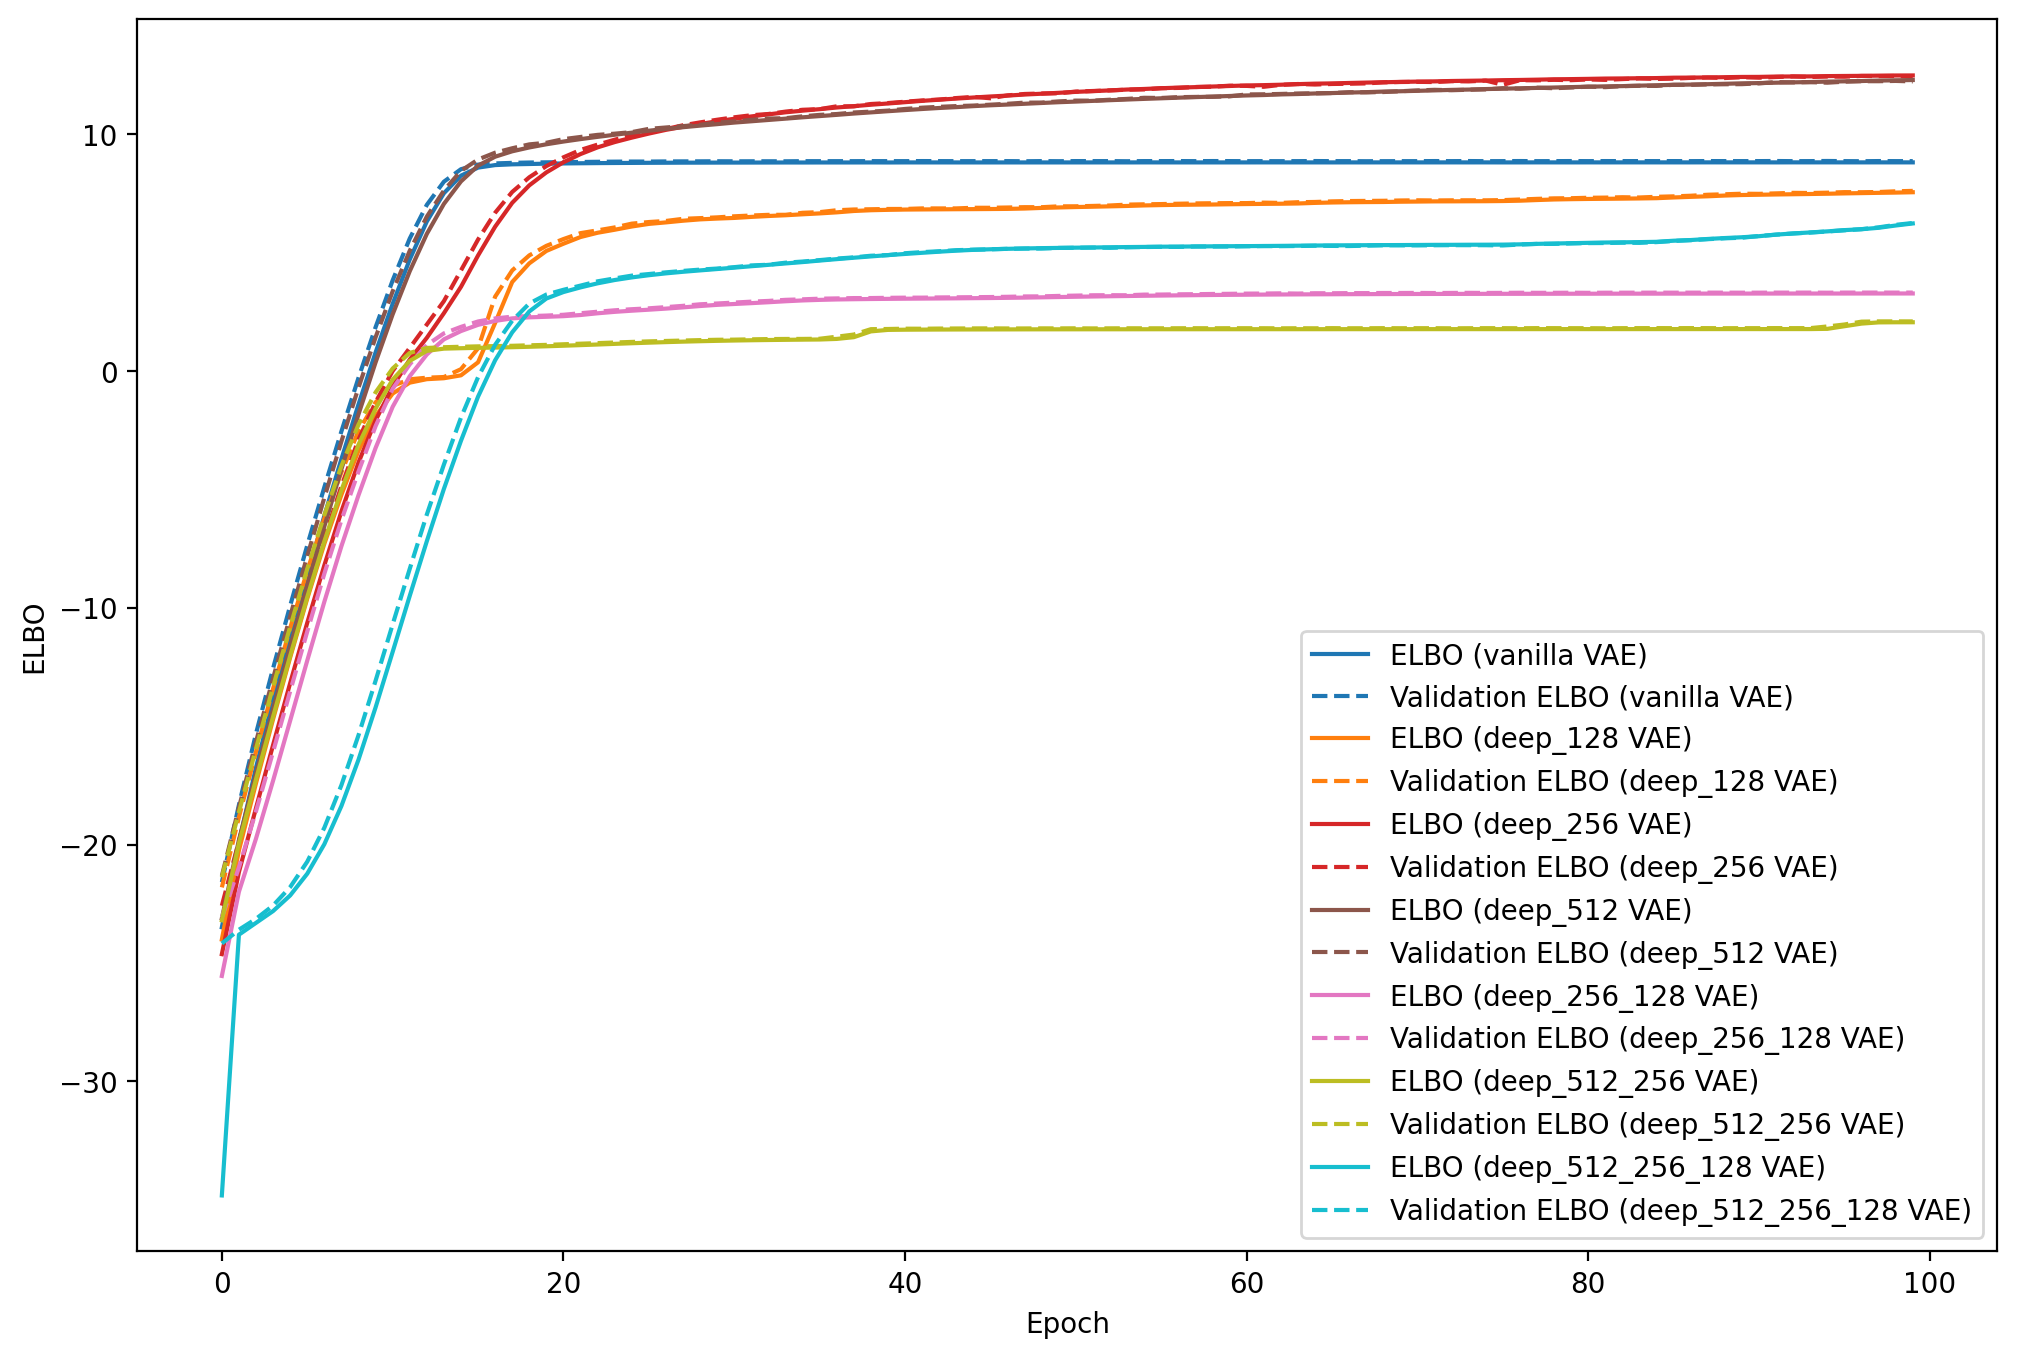
\includegraphics[width=0.8\textwidth]{../images/64_learning_curve.png}
    \caption{Learning curve for both training and validation sets for the retrained models}
    \label{fig:64_learning_curve}
\end{figure}

In this case, we can see that the learning is much more steady in the beginning but again, after around 20 epochs, the learning slows down considerably and all models follow similar trends.
Even though the most deep model shows some promising increase in ELBO in the last ten or so epochs, so if we trained for longer there could be some considerable improvements.

The number of parameters is the same as before, so we just refer the reader to Table \ref{tab:parameters}.

Again, all models were able to reconstruct the images correctly, even though the deeper models with considerably bigger blur effect.
However, we can still discern all the written digits.

\begin{figure}[ht]
    \centering
    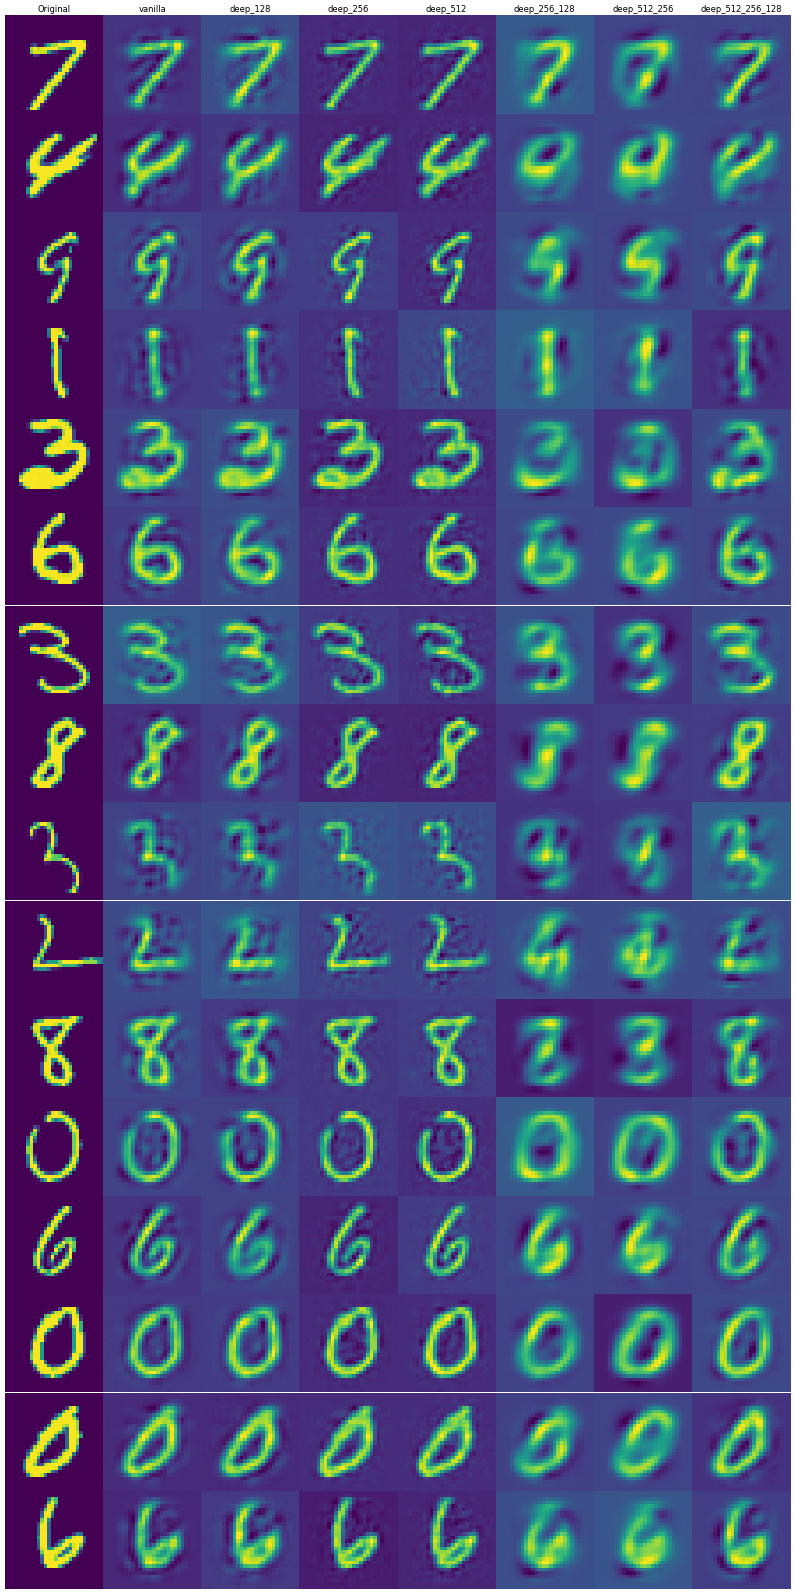
\includegraphics[width=0.45\textwidth]{../images/64_reconstructions.png}
    \caption{Reconstructed images from the test set by different retrained models. From left to right: original images, vanilla model, deep 128, deep 256, deep 512, deep 256-128, deep 512-256, deep 512-256-128.}
    \label{fig:64_reconstructions}
\end{figure}

The other comparisons of the models are a bit different.
The ELBO values in Table \ref{tab:64_elbo} show that the model with $256$ hidden units in one layer achieved the highest ELBO, which then started to drop.
However, for the deepest model, the ELBO started increasing again, so maybe some deeper model could achieve even better performance.

\begin{table}[ht]
    \centering
    \begin{tabular}{| l | c |}
        \hline
        \textbf{model}       & \textbf{ELBO} \\
        \hline
        \hline
        vanilla              & $35.92$       \\
        \hline
        deep ($128$)         & $30.90$       \\
        \hline
        deep ($256$)         & $50.14$       \\
        \hline
        deep ($512$)         & $49.26$       \\
        \hline
        deep ($256-128$)     & $13.43$       \\
        \hline
        deep ($512-256$)     & $8.52$        \\
        \hline
        deep ($512-256-128$) & $25.45$       \\
        \hline
    \end{tabular}
    \caption{ELBO values on the test set}
    \label{tab:64_elbo}
\end{table}

Posterior collapse is exactly the same situation as before, just the absolute values are a little bit different so I will omit the charts here.
But as with the previous models, the vanilla model and the model with $512$ (and here even $256$) hidden units do not have any collapsed posteriors but all of the other have some.
The deepest model has the most collapsed posteriors, which is also the majority of the dimensions.
This could mean that we could train a model with much smaller latent dimension but with more hidden hidden units to preserve the expressive value but maybe reduce the number of parameters.

The evaluation of the decoder on randomly sampled noise from $\mathcal{N}(0, 1)$ is shown in Figure \ref{fig:64_generations} and is again similar to the previous case but slightly more blurry.

\begin{figure}[ht]
    \centering
    \begin{subfigure}[t]{0.35\textwidth}
        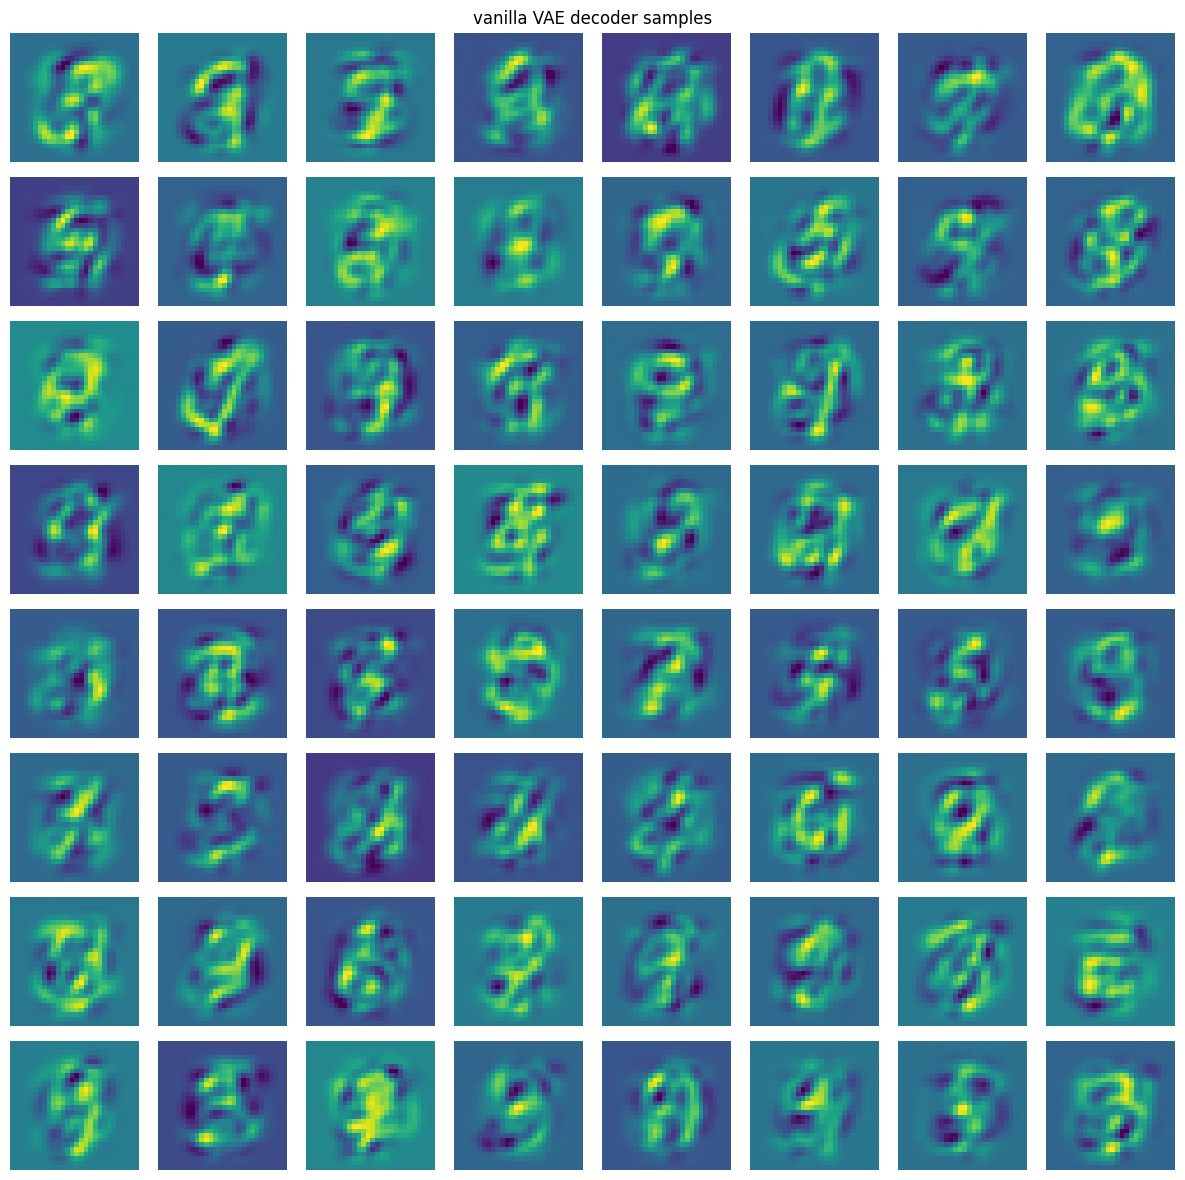
\includegraphics[width=\textwidth]{../images/64_decoder_vanilla.png}
        \caption{Vanilla model}
    \end{subfigure}
    \hfill
    \begin{subfigure}[t]{0.35\textwidth}
        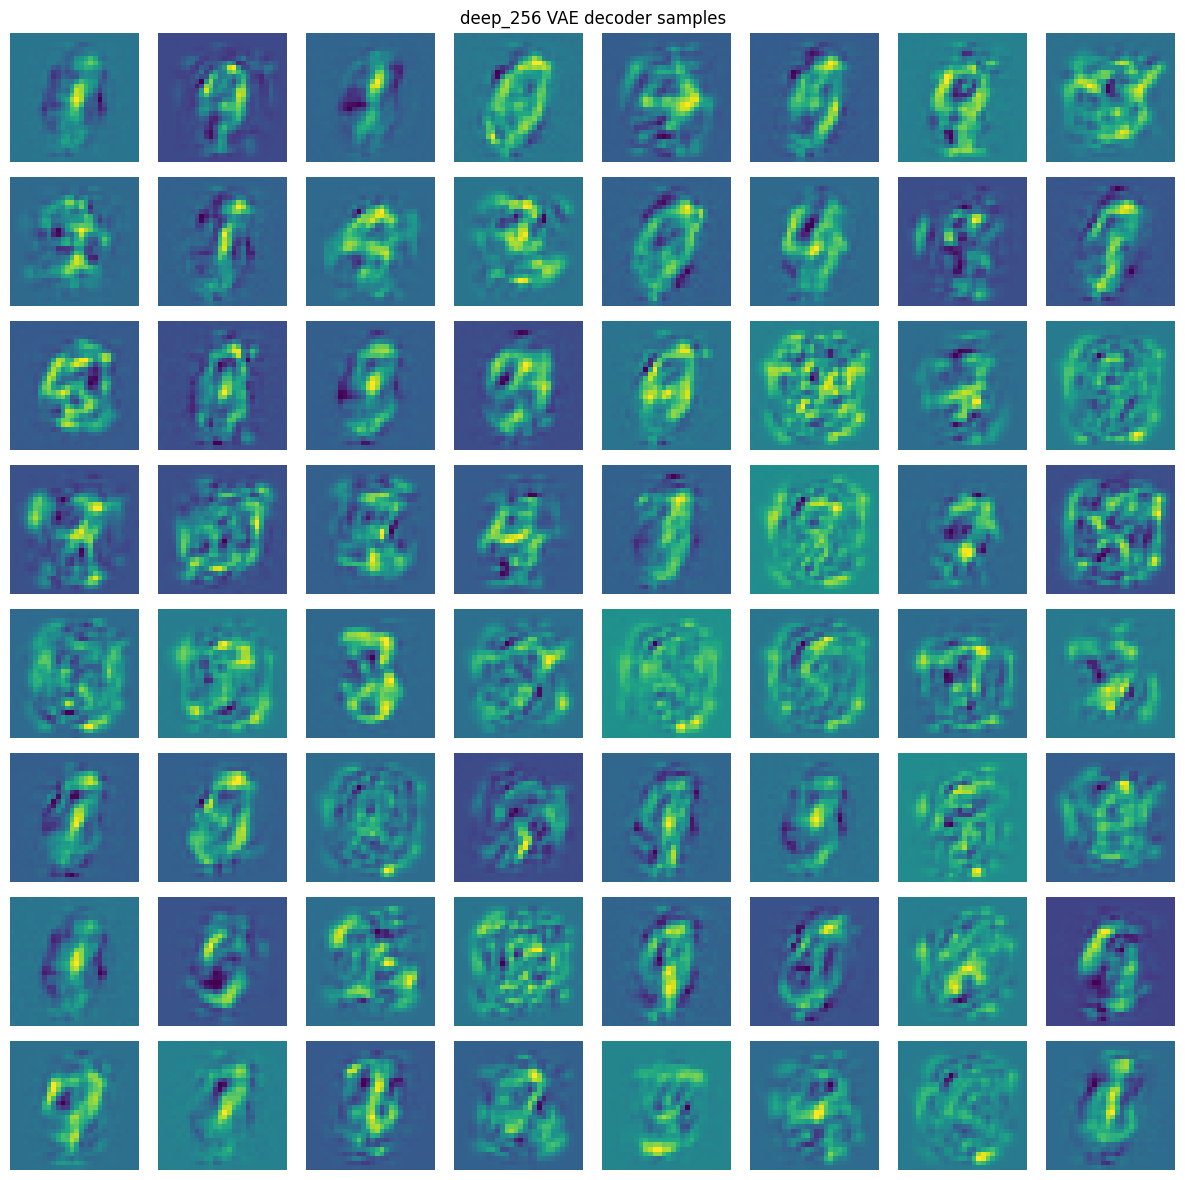
\includegraphics[width=\textwidth]{../images/64_decoder_256.png}
        \caption{Deep model with one layer and $256$ hidden units}
    \end{subfigure}
    \begin{subfigure}[t]{0.35\textwidth}
        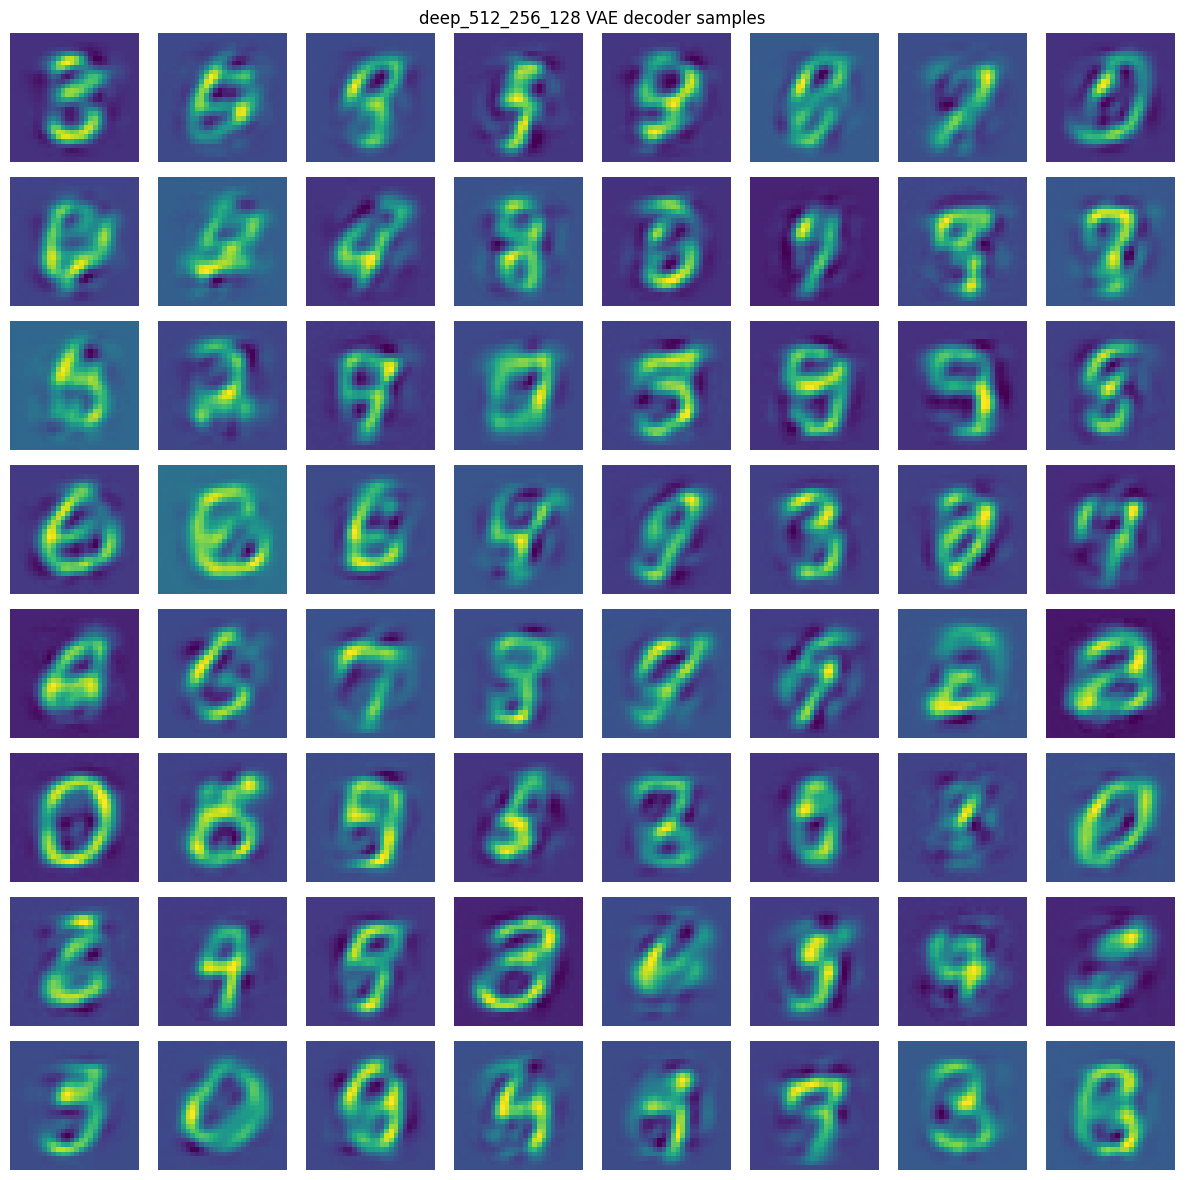
\includegraphics[width=\textwidth]{../images/64_decoder_512_256_128.png}
        \caption{Deepest model with three layers of $512-256-128$ hidden units}
    \end{subfigure}
    \caption{Images generated by decoders from $\mathcal{N}(0, 1)$ for some models}
    \label{fig:64_generations}
\end{figure}

This time, the generation of the limiting distribution was successful and the results are shown in files in the same archive as this pdf since I cannot embed them here.
I include the vanilla model, which does not do much, it has a kind of shimmering effect and sometimes one might discern something what resembles a number but not very clearly.
Then, I include the model which acheived the highest ELBO, i.e. the model with $256$ hidden units in one layer.
Lastly, I include the best performing model in terms most clear limiting distribution, which is the deepest model of them.
In this animation we can clearly see some digits, but they are sometimes morphing into another digits probably as the sampling continues.

\end{document}
